\paragraph{Versuchsziel}
Aufbau eines Pumpstandes zur Bestimmung der Evakuierungskurve und Durchführung einer
Leckratenmessung für eine Drehschieberpumpe und eine Turbomolekularpumpe
(Im Folgenden auch Turbopumpe). Daraus soll später das effektive Saugvermögen bestimmt und in
Abhängigkeit des Drucks dargestellt werden. Begleitend zum Versuch sollen die Grundlagen der
Vakuumphysik erarbeitet werden. Zudem soll man sich mit den Komponenten der Vakuumtechnik
vertraut machen. Weshalb in der Theorie \ref{sec:Theorie} auch Themen zur allgemeinen
Vakuumphysik  bzw. Vakuumtechnik besprochen werden.
\section{Theorie}
\label{sec:Theorie}
\subsection{Allgemeine Begriffserklärung}
So lange keine ausdrückliche Quellenangabe geben ist, wurde in diesem Kapitel
Quelle \cite{pfeiffer} verwendet.
\paragraph{Definition des Vakuums}
Umgangssprachlich herrscht ein Vakuum in einem Raum, wenn der Druck im Raum kleiner ist als der
Atmosphärendruck (\SI{1013}{\hecto\pascal}). Nach DIN-Norm herrscht ein Vakuum, wenn
die Teilchenzahl außerhalb größer ist als Innen oder der Druck unter \SI{300}{\milli\bar} ist.
\paragraph{Druck}
Druck ist Kraft pro Fläche. Übliche Einheiten sind Pa ,Bar ,Torr und
Psi. Dabei ist ein hPa = 100 Pa = $ 1\cdot10^{-3}$ Bar = 0,75 Torr = $1,45\cdot10^{-2}$ psi.
\paragraph{Mittlere freie Weglänge}
Die mittlere Weglänge ist die Strecke, die ein Gasteilchen ohne Stoß mit anderen Teilchen
zurücklegen kann.
\paragraph{Druckbereiche}
Es lassen sich einige Vakuumbereiche definieren, je nachdem wie stark der Unterdruck ist, ein paar
davon sind in der Tabelle \ref{tab:db} abgebildet.
\begin{table}
  \centering
  \caption{Druckbereiche der Vakuumbereiche.}
  \resizebox{\textwidth}{!}{%
  \begin{tabular}{c S@{\qquad -}S S@{\qquad-} S S@{\qquad-} S}
    \toprule
     $\text{Druckbereich}$ &
     \multicolumn{2}{c}{$\text{Druck in}\; \si{\hecto\pascal}$}  &
     \multicolumn{2}{c}{$\text{Teilchen pro}\;  \si{\cubic\meter} $}&
     \multicolumn{2}{c}{$\text{Mittlere freie Weglänge in}\;  \si{\meter} $} \\
    \midrule
    Grobvakuum & 300 & 1 & 1e19 & 1e16 & 1e-8 & 1e-4 \\
    Feinvakuum & 1&1e-3&1e16 &1e13&1e-4&1e-1\\
    Hochvakuum &	1e-3&1e-7&	1e13&1e9 &1e-1&1e3 \\
    Ultrahochvakuum & 	1e-7&1e-12 &	1e9&1e4&	1e3&1e8 \\
    \bottomrule
  \end{tabular}
}
  \label{tab:db}
\end{table}

\paragraph{Ideales Gas (Nach Quelle \cite{wiki:IG})}
Das \textit{ideale Gas} ist eine Modellvorstellung, die benutzt wird um Gase zubeschreiben.
Das Modell setzt voraus, dass die Teilchen miteinander nur durch den elastischen Stoß
wechselwirken und auch mit den Wänden elastisch Stoßen.
Dann lässt sich die ideale Gasgleichung
\begin{equation}
pV = n\symup{R}T
\label{eq:IG}
\end{equation}
aufstellen, die den Zusammenhang von Druck $p$, Volumen $V$ und Temperatur $T$ darstellt. Dabei
bezeichnet $n$ die Stoffmenge des betrachteten Gases und $R$ die allgemeine Gaskonstante.
Ein Spezialfall der idealen Gasgleichung ist das \textit{Gesetz von Boyle-Mariotte} das
besagt, dass bei konstanter Temperatur der Zusammenhang
\begin{equation*}
p \approx V^{-1}
\end{equation*}
gilt.
\paragraph{Laminare Strömung}
Bei laminarer Strömung strömen die Teilchen in gleichen zueinander parallelen Strömungsschichten.
Es treten keine Verwirbelungen, also keine turbulente Strömung, auf. Ob eine turbulente oder
eine laminare Strömung vorliegt lässt sich mit der Reynoldszahl bestimmen:
\begin{equation*}
\symup{Re} = \frac{\rho \cdot v \cdot l}{\eta} \; .
\end{equation*}
Dabei bezeichnet $\rho$ die Dichte des Fluids, $v$ die Strömungsgeschwindigkeit, $l$ die
charakteristische Länge und $\eta$ die Dynamische Viskosität des Fluids. Ist
$ \symup{Re} < 2.300 $ ist die Strömung laminar.

\paragraph{Molekulare Strömung}
Molekulare Strömung herrscht, wenn die mittlere frei Weglänge so groß ist gegen den Strömungskanals,
dass praktisch keine Wechselwirkung mehr zwischen Teilchen statt findet. Molkeulare Strömung ist
in der Regel im Bereich des Hoch- und Ultrahochvakuum vorzufinden.

\paragraph{Adsorption (Nach Quelle \cite{wiki:ads})}
Die Anreicherung von Stoffen aus Gasen und/oder Flüssigkeiten an Oberflächen von Festkörpern
bezeichnet man als Adsorption. Dabei befindet sich das Gas oder die Flüssigkeit im Allgemeinen
im Übergang zwischen zwei Phasen.

\paragraph{Absorption (Nach Quelle \cite{wiki:abs})}
Die Aufnahme eines Atoms, Moleküls oder Ions in einer anderen Phase, in das freie Volumen der
absorbierenden Phase, bezeichnet man als Absorption. Es handelt sich hier also nicht nur
um eine Anlagerung an der Oberfläche, wie bei der Adsorption.

\paragraph{Desorption}
Ist die Abgabe von Gasmolekühle, die sich vorher durch Ab- und Absorption an Flächen abgereichert
haben. Dies führt beim Anlegen eines Vakuums, zu einem Gasanfall im Rezipienten (= Raum in dem
das Vakuum herrschen soll).

\paragraph{Diffusion (Nach Quelle \cite{wiki:dif})}
Ist der Ausgleich zwischen Konzentrationsunterschiede aufgrund der brownschen Molekularbewegung.
In der Vakuumphysik tritt dieses Phänomen ebenfalls als Gasanfall im Rezipienten auf, wenn
ein Vakuum angelegt ist.
\paragraph{Virtuelle Lecks (Nach Quelle \cite{wiki:vl})}
Virtuelle Lecks haben ähnliche Effekte wie reale Lecks. Sie entstehen durch Diffusion, Desorption
aus den Wänden des Rezipienten (z.B. aus Gaseinschlüssen in Schweißnähten) oder durch Rückstände
von der Fertigung.

\subsection{Vakuumtechnik}
\paragraph{Vakuumpumpe (Nach Quelle \cite{pfeiffer})}
In der Vakuumtechnik unterscheidet man zwischen gasfördernen und gasbindenen Pumpen. Die
gasfördernen Pumpen werden noch einmal unterschieden
in Verdrängerpumpen und kinetische Vakuumpumpen.
Verdrängerpumpen evakuieren den Rezipienten indem sie das Gas herausfördern. Kinetische
Vakuumpumpen befördern das Gas entweder durch Beschleunigung der Gasteilchen in Pumprichtung oder
durch einen Dampfstrahl, der dann kondensiert wird. Gasbindende Pumpen binden das Gas durch
Physisorption, Abkühlung auf niedrige Temperaturen oder Chemisorption an Oberflächen.
Die in diesem Versuch verwendeten Vakuumpumpe sind beide gasfördernde Pumpen. Wobei
die verwendete Drehschieberpumpe eine Verdrängervakuumpumpe ist und die Turbomolekularpumpe
eine kintetische Vakuumpumpe ist.

\paragraph{Drehschiebervakuumpumpe (Nach Quelle \cite{pfeiffer})}
Die Drehschieberpumpe besteht, wie in Abbildung \ref{fig:dp} abgebildet aus einem Gehäuse (1)
auch Stator genannt, einem
Rotor der exzentrisch eingebaut ist (2), in diesem Rotor ist der Schieber eingebaut der mit einer
Feder an das Gehäuse gedrückt wird. Aus und in den Arbeitsraum (5) führt der Aus- und Einlass (4).
Der Schieber teilt den Arbeitsraum in zwei Räume. Fährt der Schieber nun am Einlass vorbei
strömt das Gas in das "neu" entstandene Volumen. Nach dem der darauf folgende Schieber das Volumen
abschließt wird das Gas, welches zwischen den zwei Schiebern nun gefangen ist komprimiert.
Ist der Druck des Gases nun groß genug gegen über den Außendruck öffnet sich das Auslassventil (6)
und das Gas strömt in den Auslass. Dabei wird aus dem Auslass eine kleine Menge Öl in den
Arbeitsraum gegeben, dies Schmiert nicht nur sondern dichtet auch die Grenze zwischen Schieber und
Stator ab. Eine Drehschiebervakuumpumpe wird verwendet um ein Vakuum mit ca. \SI{300}{\hecto\pascal}
zu erzeugen.


\begin{figure}
  \centering
  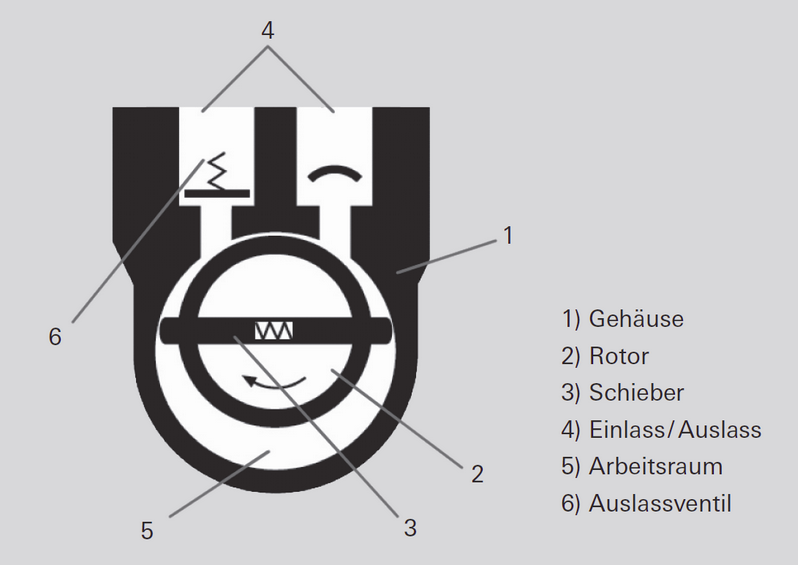
\includegraphics[height = 7cm]{pics/dp.png}
  \caption{Schematische Darstellung des Funktionsprinzips einer Drehschieberpumpe \cite{pfeiffer:dp}.}
  \label{fig:dp}
\end{figure}
\FloatBarrier

\paragraph{Turbomolekularvakuumpumpe}
Die Turbomolekularpumpe besteht, wie in Abbildung \ref{fig:stm} zu sehen, aus aufeinander folgenden
Stator und Rotorblättern. Das Prinzip besteht darauf, dass den Gasteilchen soviel Impuls
übergeben wird, dass sie auf die Statorblätter treffen und abtransportiert werden können. Dafür
muss in der Pumpe selbst molekulare Strömung vorliegen. Zudem sollte die
mittlere frei Weglänge größer sein als der Abstand der Rotorblätter. Deshalb muss das Vakuum im
Rezipienten bei ca. \SI{10}{\hecto\pascal} liegen.

\begin{figure}
  \centering
  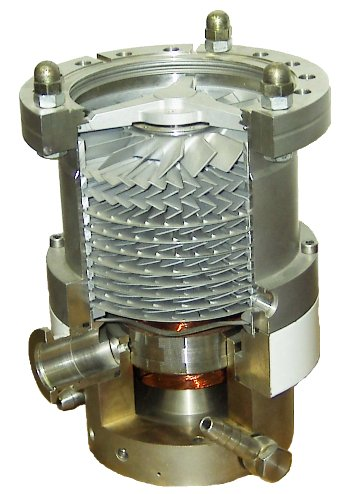
\includegraphics[height = 5cm]{pics/tm.jpg}
  \caption{Schnitt durch eine Turbomolekularpumpe aus Quelle \cite{wiki:tm}.}
  \label{fig:stm}
\end{figure}
\FloatBarrier

\paragraph{Pirani-Vakuummeter (Nach Quelle \cite{pfeiffer:mg})}
Das Pirani-Vakuummeter bestimmt den Druck des Gases über die Wärmeleitfähigkeit. Der Messbereich
liegt daher ca. im Bereich zwischen 10 bis \SI{10e-4}{\hecto\pascal}, da die Wärmeleitung
über \SI{10}{\hecto\pascal} druckunabhängig ist und ab \SI{10e-4}{\hecto\pascal} die Wärmeleitung
aufgrund des Aufbaus nur noch ein schwacher Indikator ist. Das Pirani-Vakuummeter besteht aus einem
Draht in einem Rohr, der auf ca. \SI{100}{\degree} erwärmt wird. Die Wärme des Drahtes wird über
die Gasteilchen auf die Rohrwand abgeleitet. Der Wärmetransport ist dann proportional zum Druck,
solange die Temperatur des Drahtes konstant gehalten wird.

\paragraph{Kaltkathoden-Ionisationsvakuummeter (Nach Quelle \cite{pfeiffer:mg})}
Das Kaltkathoden-Ionisationsvakuummeter besteht aus einer Kathode und einer Anode, an denen eine
Hochspannung angelegt ist. Durch Feldemission lösen sich Elektronen aus der Kathode und ionisieren
auf dem Weg zu Anode die Gasteilchen, um diesen Effekt zu verstärken wird zusätzlich ein
Magnetfeld angelegt um den Weg der Elektronen zu verlängern. Die Ionisation der Gasteilchen
führt zur Gasentladung, die wiederum zu einem Gasentladungsstrom. Vom Gasentladungsstrom
kann auf den Druck geschlossen werden.

\paragraph{Heißkathoden-Vakuummeter (Nach Quelle \cite{pfeiffer:mg})}
Bei diesem Vakuummeter werden die Elektronen durch eine Heißkathode emittiert. Auf ihren Weg
ionisieren sie Gasteilchen. Die Anode ist zylindrisch und gitterförmig und in ihrer Mitte befindet
sich ein Draht, dieser ist Auffänger für die Ionen die durch Stoßionisation entstehen. Der
Ionenstrom ist dann Maß für den Druck. Mit diesem Messgerät lässt sich Druck bis zu
\SI{10e-10}{\hecto\pascal} bestimmen. Ein Beispiel eines Heißkathoden-Vakuummeters ist die
Messröhre nach Bayard-Alpert, ein schematischer Aufbau ist in der Abbildung \ref{fig:bam} zu
betrachten.
\newline
Sowohl das Heißkathoden-Vakuummeter als auch das Klatkathoden-Ionsisationsvakuummeter wird erst ab
einem Druck von \SI{10e-3}{\hecto\pascal} verwendet, da es bei höheren Drücken durchbrennen oder
verschmutzen würde.

\begin{figure}
  \centering
  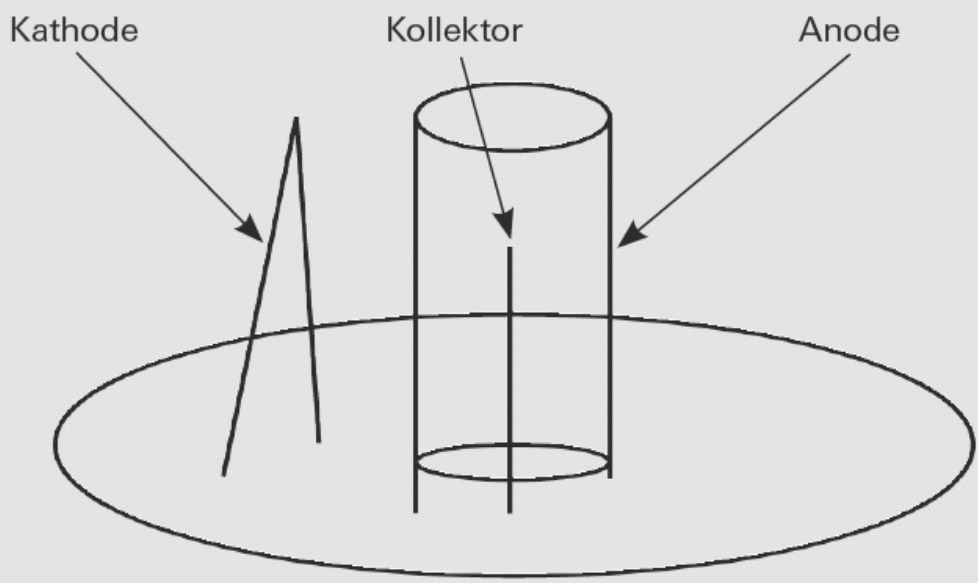
\includegraphics[height = 5cm]{pics/bam.png}
  \caption{Schematischer Aufbau einer Bayard-Alpert Messröhre aus Quelle \cite{pfeiffer:bam}.}
  \label{fig:bam}
\end{figure}
\FloatBarrier
\subsection{Bestimmung des Saugvermögen aus p(t)-Kurven (Nach Quelle \cite{Anleitung})}
Zur Bestimmung des Saugvermögens müssen zu erst folgende Annahmen getroffen werden
\begin{itemize}
\item Das Volumen $V$ ist konstant, während der Druckmessung
\item Das Gas kann mit dem Modell des idealen Gases beschrieben werden
\item Die Messung verlief bei konstanter Temperatur $T$
\item Das Gas ist zu jedem Zeitpunkt im thermodynamischen Gleichgewicht
\item Lecks und Effekte der Desorption sind zu vernachlässigen
\item Das Saugvermögen $S$ ist konstant und unabhängig vom Druck $p$
\end{itemize}

Mit dem einfachsten Modell einer Pumpe (Kolbenpumpe), kann dann angenommen werden, dass
$ \dot{V} = S $ gilt. Leitet man nun die ideale Gasgleichung \eqref{eq:IG} einmal nach der Zeit ab
folgt die Gleichung
\begin{equation*}
\dot{p}V = -pS \; ,
\end{equation*}
dabei ist zu beachten, dass die Temperatur als konstant angenommen wurde. Die so entstandene
Differentialgleichung lässt sich mit dem Ansatz
\begin{equation*}
p(t) = p:0 \symup{exp}\left( -\frac{t}{\tau} \right)
\end{equation*}
mit Anfangsdruck $p_0$ lösen. Durch einsetzen ergibt sich dann $ \tau = \sfrac{V}{T} $.
Berücksichtigt man nun noch das es einen endlichen Enddruck $p_E$  gibt, folgt die Gleichung
\begin{equation}
p(t) = (p_0 - p_E) \cdot \symup{exp}\left( -t \frac{S}{V} + p_E \right) \; .
\label{eq:pt}
\end{equation}
Die Tatsache, dass es einen Enddruck geben muss folgt allein daraus, dass Effekte wie
Desorption, reale und virtuelle Lecks auftreten. Aufgrund der Funktionsweise der Pumpen kann
ebenfalls nur ein endlicher Enddruck erreicht werden, da Effekte wie Rückströmung, Totvolumen
sowie ein endliches Kompressionsvermögen vorliegen.

\paragraph{Leckratenmessung}
Die Leckrate $Q$ gibt an wieviel Gas pro Zeit aus dem Aufbau leckt. Es gilt der Zusammenhang
\begin{equation*}
 S=  \frac{Q}{p_g} \qquad \text{mit} \qquad Q = V\cdot \frac{\symup{d}p}{\symup{d}t}\;.
\end{equation*}
Dann folgt für das Saugvermögen
\begin{equation}
S = \frac{V}{p_g} \cdot \frac{\symup{d}p}{\symup{d}t} \; ,
\label{eq:SQ}
\end{equation}
damit lässt sich aus eine Leckratenmessung das Saugvermögen $S$ bestimmen.

\paragraph{Leitwert}
Aufgrund von Strömungswiderständen der Verbindungsstücke, kann die Angabe des Herstellers für
das Saugvermogen $S_0$ nicht erreicht werden. Deshalb definiert man ein effektives Saugvermögen
durch
\begin{equation}
\frac{1}{S_{eff}} = \frac{1}{S_0} + \frac{1}{L} \; .
\label{eq:Seff}
\end{equation}
Das effektive Saugvermögen, auch Nennsaugvermögen der Pumpe am Ansaugstuzen genannt, ergibt sich
aus dem Kehrwert der Herstellerangabe und dem Kehrwert des Leitwerts. Der Leitwert ist der
reziproke Strömungswiderstand der Verbindungen.
